%%Main takeaway - we provide calving front locations, and have automated it
%Some may be more interested in the data, or the method, so make sure we cover both

\documentclass[tc, manuscript]{copernicus}

\usepackage{wrapfig}
\usepackage{amsmath}
\DeclareMathOperator*{\argmax}{arg\,max}
\DeclareMathOperator*{\argmin}{arg\,min}

\begin{document}

\title{Calving Front Machine (CALFIN): Automated Calving Front Mask Dataset and Methodology for East/West Greenland, 1972-2019}

\Author[1]{Daniel}{Cheng}
\Author[1]{Yara}{Mohajerani}
\Author[1]{Isabella}{Velicogna}
\Author[2]{Eric}{Larour}
\Author[1]{Wayne}{Hayes}

\affil[University of California at Irvine]{Irvine CA, USA}
\affil[Jet Propulsion Laboratory, California Institute of Technology]{Pasadena CA, USA}

\runningtitle{TEXT}

\runningauthor{TEXT}

\correspondence{Daniel Cheng (dlcheng@uci.edu)}

\received{}
\pubdiscuss{} %% only important for two-stage journals
\revised{}
\accepted{}
\published{}

\maketitle

\begin{abstract}
We present Calving Front Machine (CALFIN), a dataset of calving front masks for glaciers along West Greenland. The dataset is generated from Landsat imagery over the period 1972 to 2019. This dataset is unique in scope, and provides new constraints on glacial evolution over the time period. The current iteration offers a new opportunity to explore previous trends and validate existing models, enabling more accurate predictions moving forward.

The dataset is contains data that is automatically generated. We generate the vectorized calving fronts from raw Landsat imagery. Our method utilizes deep learning in the form of a neural network. This approach builds on existing work \cite{mohajerani-rs} \cite{zhang-tc} \cite{baumhoer}. The network itself is derived from U-Net/DeeplabV3+ Xception architectures \cite{unet} \cite{deeplabv3+} . Additional post-processing techniques allow our method to achieve accurate and useful segmentation of raw images into Shapefile outputs. This methodology is uniquely robust to clouds, illumination differences, ice mélange, and Landsat-7 scanline errors/data coverage gaps.

We perform an analysis of CALFIN results, which approach human levels of accuracy in comparison to manually delineated fronts. Additionally, we perform a model inter-comparison to evaluate the robustness of CALFIN's performance and cross-validate it against existing methodologies. %TODO/Save for future paper? We show the applicability of CALFIN's methodology to SAR data, Antarctic glaciers, as well as non-marine terminating glaciers.

At this stage, we seek feedback from the community and welcome any critiques or questions regarding the dataset and/or our methods. This work was conducted as a collaboration between NASA’s Jet Propulsion Laboratory and the University of California, Irvine.
\cite{edge-detection}
\cite{texture-analysis}
\cite{unet}
\cite{teranus-carvana}
\cite{xception}
\cite{deeplabv3}
\cite{deeplabv3+}
\cite{bjork-names-tc}
\cite{mohajerani-rs}
\cite{zhang-tc}
\cite{baumhoer}
\cite{esa-cci-cfl}
\end{abstract}

\introduction
%Introduction
The evolution of Greenland's tidewater glaciers is an important constraint on the evolution of the Greenland Ice Sheet as a whole. Likewise, changes in the Greenland are important in tracking and predicting changes in the climate overall. Constraining Greenland's glacial evolution is thus an important part of improving our understanding of Earth's climate.

%Comment out subsection headers?
\subsection{Motivation}
One such constraint on glacial evolution is the position of glacial calving fronts over time. However, delineating the calving fronts of marine-terminating glaciers is typically a time-intensive manual process. As a result, many glaciers receive less labeling than is ideal, or none at all. Additionally, existing glaciers that do receive annual labeling do not capture intra-annual variability. 

The need for an improved methodology is apparent. An automated methodology allows for the solution to previously stated issues. However, the automation of glacial calving front delineation is non-trivial. Confounding issues - such as cloud cover, ice mélange, shadowing,  - present an impediment to naive techniques such as edge detection and texture analysis. Ultimately, emerging techniques in computer science provide a promising approach to this problem. More specifically, machine learning and deep neural networks provide a robust, scalable, and accurate method to automatically delineate tidewater glacial calving fronts.

\subsection{Methodology}
In this study, we evaluate automated methods of delineating glacial termini. The glaciers studied are located along East/West Greenland. They include Helheim, Kangerlussuaq, Kong Oscar, Hayes, Rink Isbrae, Upernavik, Jakobshavn, Kangiata Nunata, and 58 other nearby glaciers. The intra-annual time series studied spans from 1972 to June 2019. Our source data is the Landsat Near Infrared (NIR) band.

We determine that convolutional neural networks present the most promising automated methodology. We determine that the UNet-inspired DeeplabV3+ architecture, with Xception backbone, is the most promising neural network architecture. We release a modified version of the DeeplabV3+ network, along with the final weights we use for data production. We release a set of data products, Calving Front Machine (CALFIN), which consists of both calving front masks as well as Shapefile polylines for the 88 glacial basins along East/West Greenland.

\subsection{Existing Work}
Existing efforts have been made by ESA's climate Change Initiative to provide calving front locations for 26 Greenlandic basins, from 1990-2016\cite{esa-cci-cfl}. Additionally, there are growing efforts to provide a unified database of manually delineated calving fronts. Nonetheless, the constant addition of new data, as well as the current scarcity of shared data, implies a consistent and repeated need for new data assimilation efforts.

We evaluate existing work in the field, performed by Yara Mohajerani, Enze Zhang, and Celia Baumhoer. These studies offer the potential to cross-validate the viability of our own methods.

\subsection{Takeaways}
Our main takeaway is the viability of generalized neural networks for automated calving front detection. Specifically, a well trained network is able to approach human levels of accuracy in picking out arbitrary glacial calving fronts. This demonstration of learning also lends credence to this methodology as a viable approach to other data assimilation tasks.

Our key goal is to provide high spatial accuracy, dense temporal resolution, and long time series calving front masks for the cryospheric/climate modeling community. We look forward to fulfilling this goal as we continue to improve our methods and release additional data moving forward.

\section{Data - Source and Preprocessing}
\subsection{Data - Source}
We evaluated several potential dataset sources that would provide the raw data from which we would assimilate calving front positions.

Name            Resolution(s)       Time Series     Sensor  
Landsat         30m, 60m            1972-present    Optical
Terra (MODIS)   250m, 500m, 1000m   1999-present    Optical
Sentinel        10m, 20m, 60m       2014-present    SAR
TerraSAR-X      1m, 3m, 6m          2007-present    SAR

We chose Landsat due to the combination of long time-series availability and reasonable spatial resolution. The time period we study spans from 1972 to June 2019.


We decided to constrain our input to be based on subsets of a single band. Part of this was due to computational constraints, as larger inputs result in longer processing times and hardware requirements. Another part of this was due to diminishing returns from adding additional bands. Since pixel information can be correlated across different bands, and since a single band image already shows any discernible calving fronts, additional band information was deemed unnecessary.


\begin{figure}[t]
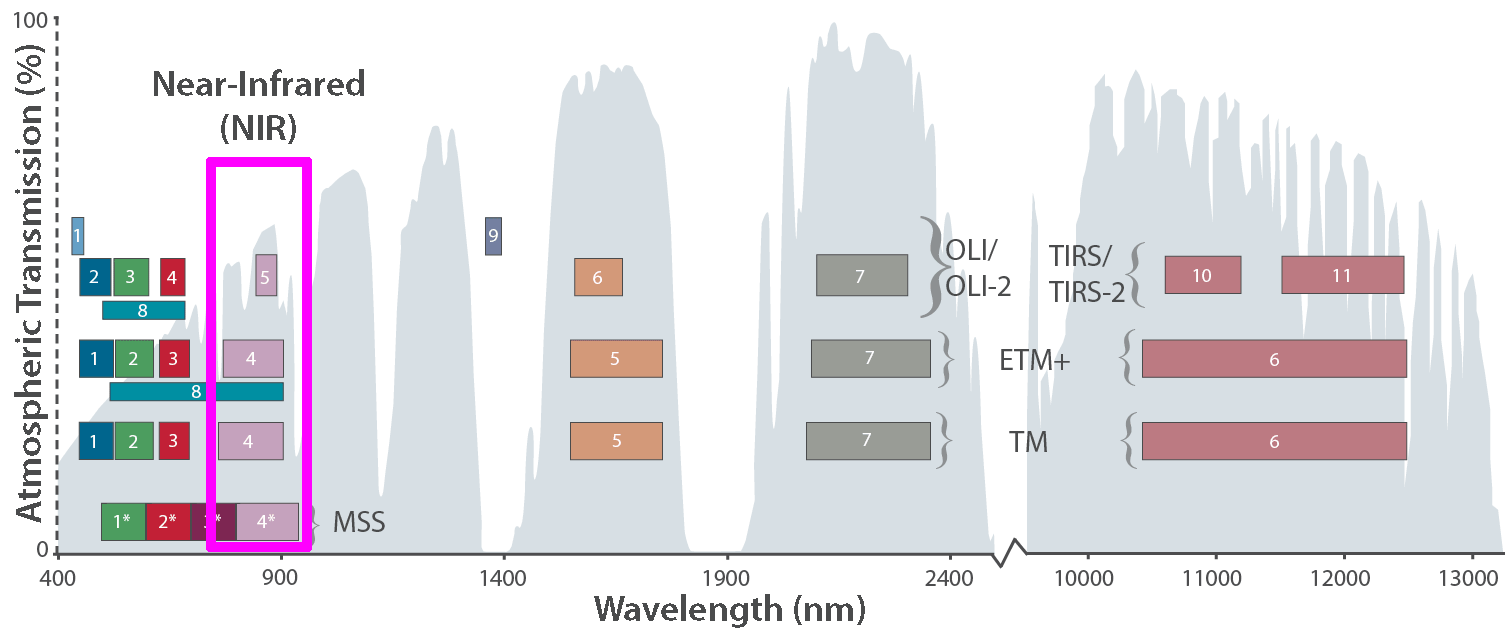
\includegraphics[width=17cm]{all_Landsat_bands_annotated.png}
\centering
\end{figure}
%Insert landsat band overlap table
%https://landsat.gsfc.nasa.gov/landsat-9/landsat-9-spectral-bands/
We picked the Near Infrared (NIR) (.77-1.1um) wavelength band. This was based on evaluating  Landsat 1 - 8 band commonality, and atmospheric water transmittance -allowing us to "look past" light cloud cover. We hypothesize that using a common band is beneficial, as different spectral bands may exhibit features differently, and thus negatively impact detection accuracy.




%%FIX THESE FIGURES - UPDATE TEMPORAL RESOLUTION & ADD TO SPATIAL COVERAGE MAPS

\subsubsection{Time Series Coverage}
-Landsat availability per year, for all 6 basins.
- Additional gaps due to clouds or lack of classifier confidence
- Color key shows rough number of observations per year

\begin{wrapfigure}{r}{0.3\textwidth} %this figure will be at the right
    \centering
    \includegraphics[width=0.3\textwidth]{time-coverage.png}
    \caption{Number of images across the years for 6 glaciers.}
\end{wrapfigure}


\subsubsection{Spatial Coverage}
- CALFIN data availability along West Greenland, for the highlighted basins, over velocity map (Naglar, 2015)1
- Basins selected for equal sampling of coastline
- Basins selected for study potential/high velocities

\begin{wrapfigure}{r}{0.4\textwidth} %this figure will be at the right
    \centering
    \includegraphics[width=0.4\textwidth]{spatial-coverage.png}
\end{wrapfigure}



\subsection{Data - Preprocessing}
Throughout our study, we developed pipeline that automates much of the data preprocessing that is required for this task. Currently, each step can operate 

\subsubsection{Data - Preprocessing - Collection}
As a first step, we collect the input raster images that for which we want to evaluate. We utilize all available input image time steps with less than 20\% cloud cover across the entire area. We accumulate 4776 Landsat rasters, from which we subset individual glacial domains. 

\subsubsection{Data - Preprocessing - Subsetting}
To begin subsetting, we define the domain of a glacial basin, which should fully encloses the calving front being extracted. We encode the domain as a rectangular Shapefile polygon. Next, we automatically subset the raster for every time step which we want to evaluate for the domain. We repeat this process for each basin to be studied. While this requires manual input, it only needs to be done once, as the domains will be reused across multiple subsetting operations.
%For rasters and domains in West Greendland, we reproject to WGS 84 / UTM zone 21N (EPSG:32621). For East Greenland, we use WGS_1984_UTM_Zone_24N (EPSG:32624)

\subsubsection{Data - Preprocessing - Pruning}
After subsetting, we automatically prune images that are ill-suited for further processing. First, we determine the amount of NODATA pixels present in the subset, and remove it from evaluation if it exceeds a predetermined threshold (>30\%). This allows us to process images with Landsat 7 scanline errors and domains along raster boundaries, while still filtering out largely out-of-bounds subsets. This prevents them from being unnecessarily and inaccurately processed. Also, if an accompanying Quality Assurance band is present, the same filtering procedure is performed to eliminate images with high cloud cover, for the same reasons. We accumulate 20,029 image subsets, spread across 66 glacial domains.

\subsubsection{Data - Preprocessing - Standardization}
Then, we resize the image to a standardized, square resolution. We convert the subsets from their native GeoTIFF formats to a standardized 256x256 PNG image. While larger networks The GeoTIFF subsets are utilized for rescaling and georeferencing the Shapefile after processing. This step can introduce error into the delineation, which we address by defining domains as close to the specified square resolution whenever possible.
%We found through empirical testing that this input resolution is optimally balanced considering accuracy of the output and computational bottleneck. 

\subsubsection{Data - Preprocessing - Detail Enhancement}
Lastly, we perform image transformations to enhance detail and provide the processing step with more information. We found through empirical testing that this step specifically benefits raw images with heavy shadowing. This benefit emerges since these images contain details which are otherwise undetectable by the filters used in the processing step. We utilize two non-linear transformations, the Pseudo-HDR Toning and Shadows and Highlights enhancements. These enhancements are performed with default settings in Adobe Photoshop, but we aim to write an open-source equivalent in Python. We concatenate the results of the two transformations with the raw image. This creates 3-channel RGB input images that contains information that can be utilized by the next step. 

At this point, the images are ready for processing into calving front masks.

%Jumping to final implementaiton - should we fill in-between networks? Probably should skip to here - no sense in covering everything that was done, too long
%NOTE: I moved the edge detection/texture analysis/neural network explanation down and commented it out for now
\section{Methodology - Processing}
We perform the core processing step by passing images through the Calving Front Machine Neural Network (CALFIN-NN). As a convolutional neural network that inherits from the U-Net family of architectures, CALFIN-NN is capable of learning abstract image features, and generalizes to new data automatically. This key capability is the foundation of most other automated methods in this field, including those by Zhang \cite{zhang-tc}, Mohajenrani \cite{mohajerani-rs}, and Baumhoer \cite{baumhoer}. Our network builds upon this work, and utilizes a modification of Google's Depplabv3+ Xception image segmentation network. With our customized architecture and training regimen, CALFIN-NN is capable of handling inputs with different scales/resolutions, heavy shadowing, ice mélange, light cloud cover, and Landsat 7 scan-line errors. Together, these novel innovations bring the  state-of-the-art in image segmentation to the cryosphere community. The following section describes the details of our network model, including the iterative process of testing, evaluation methods, and our final training regimen.

\subsection{Methodology - Processing - Model Architecture \& Details}
CALFIN-NN takes in 3-channel preprocessed images, and outputs 2-channel images containing the edge and the land ice/ocean mask. 


\begin{figure}[t]
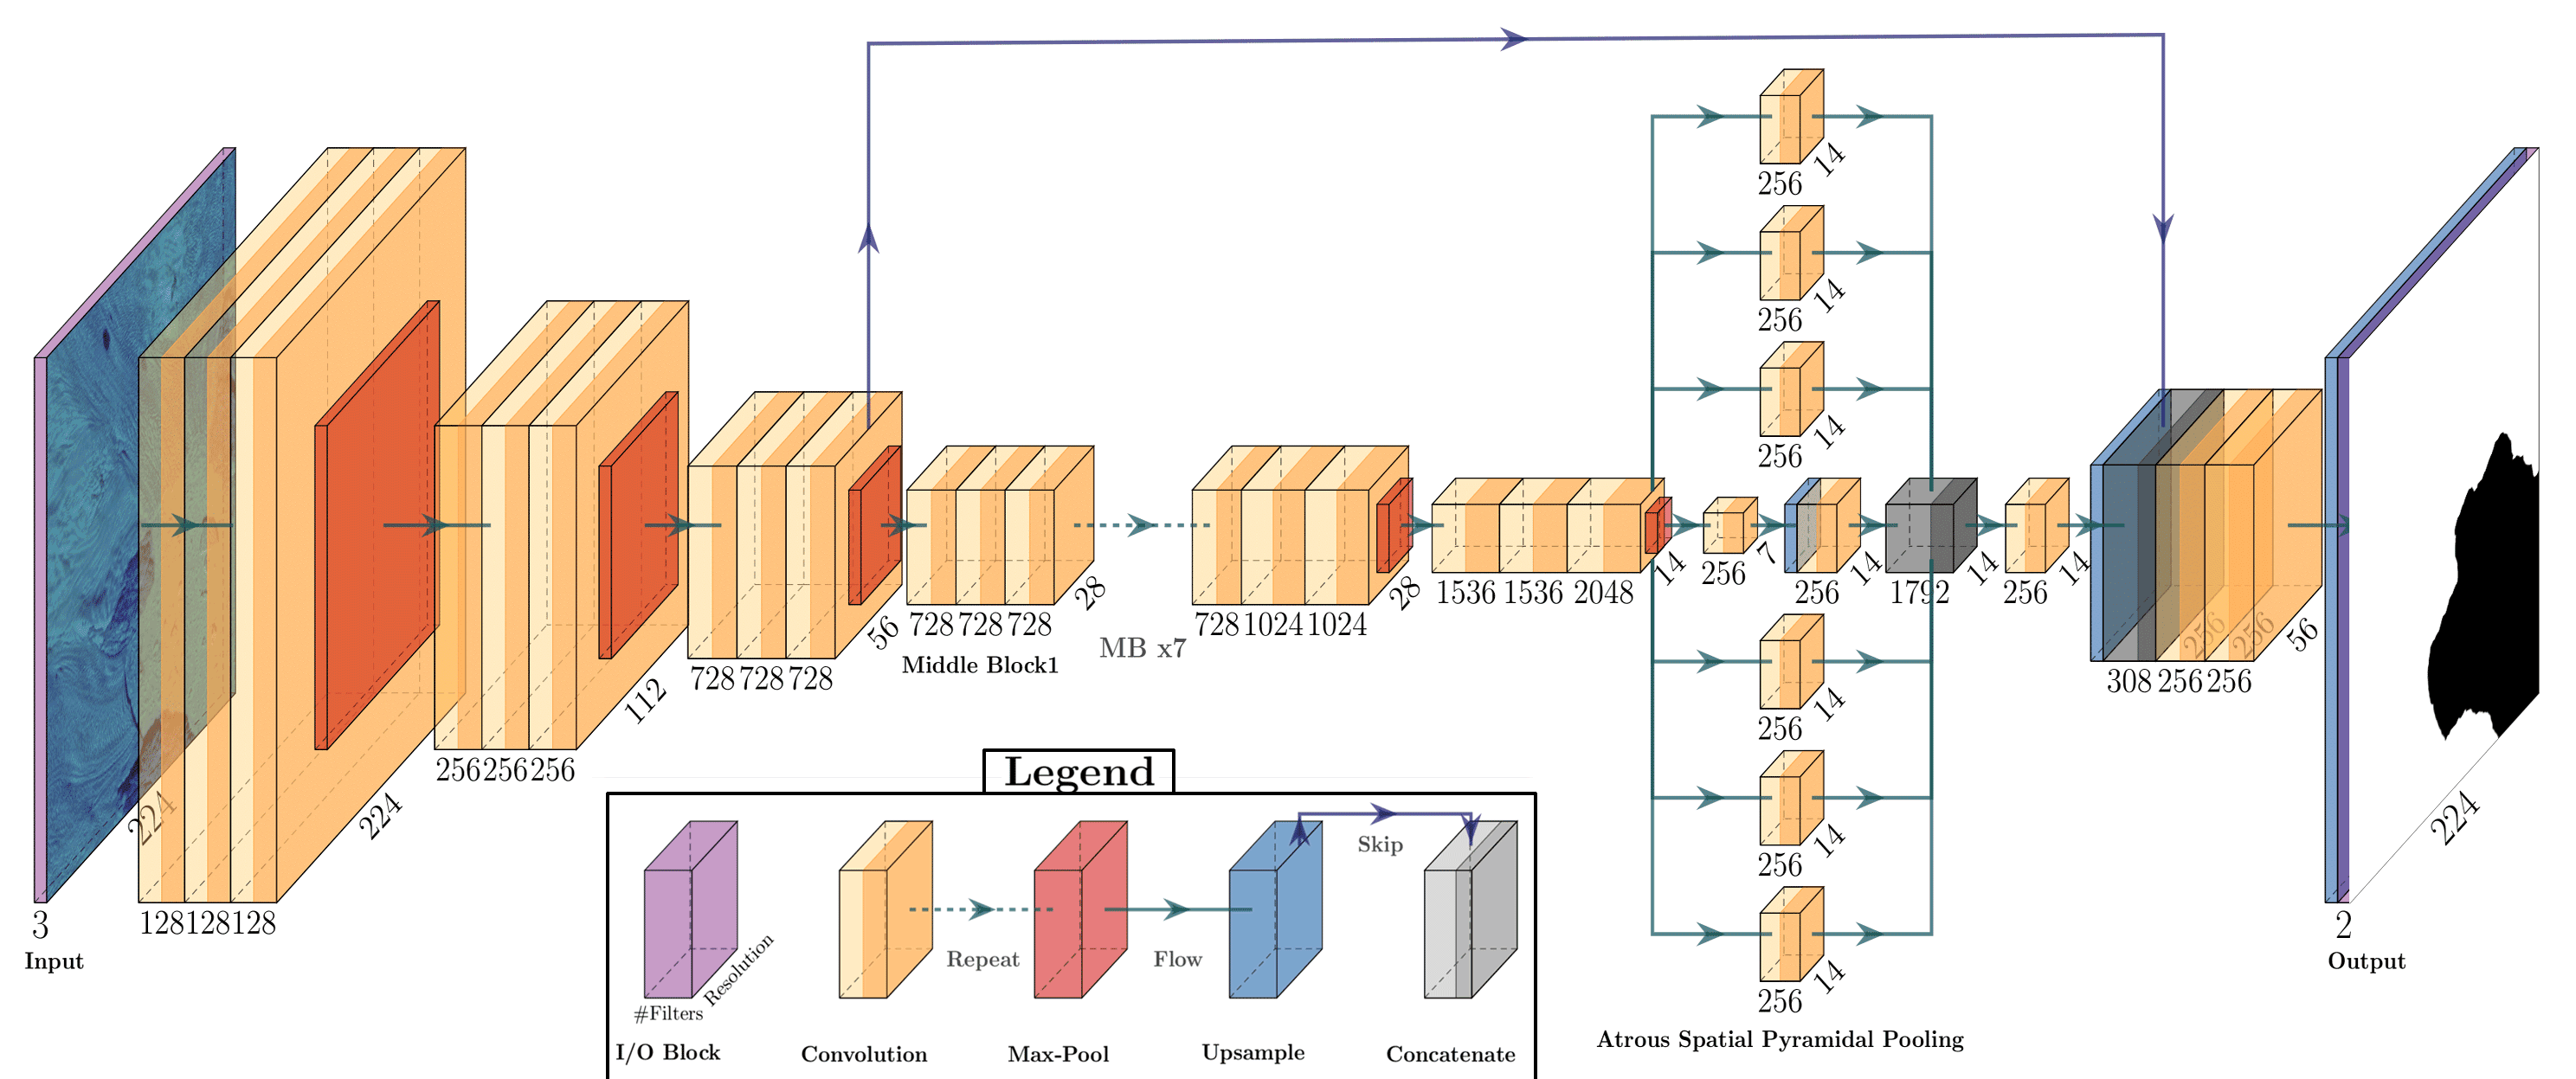
\includegraphics[width=18cm]{arch_final.png}
\centering
\end{figure}
%FIGURE HERE: CREATE NETWORK FIGURE

%List out features of Deeplab first
-Xception modules and Atrous Spatial Pyramidal Pooling capture multiscale features
-Built for image segmentation/classification, but needs work for recognizing thin/line like features like calving fronts

%List modifications to the above
-Modification of the 6, 12, 18 ASPP branches to 1, 2, 3, 4, 5
-Usage of Xception 65 layer base implementation instead of default header module in Deeplabv3+
-Modified output: 2 channel output for mask and edge simultaneously
-Reduced weight size: 29m parameters, ~400MB


%Features
-224x224 image size: 
-3 channel input: Our network intakes a 3 channel image input.
    -R channel: Raw image, directly taken from the Landsat domain subset.
    -G channel: High-Definition Range Toning image, processed in Adobe Photoshop.
    -B channel: Shadows and Highlights enhancement image, processed in Adobe Photoshop
-2 channel output:
    -R channel: Edge mask. 
    -G channel: Ice/ocean mask.


%Show an image here?
%Problem: low accuracy with higher resolution.
Solution: We remade our training data at higher resolutions and enlarged the edges of the detected fronts to address scaling issues. Effectively, we made a larger target, and thus made it easier to achieve, without sacrificing accuracy.

%Problem: Memory-effects/overfitting.
Solution: We added data augmentation to enforce learning more general features. These included image translation, noise addition, and detail-preserving image filters like emboss/CLAHE.

%Problem: Validation accuracy did not reflect test accuracy.
Solution: We added additional training images from all 60 additional domains, including some from East Greenland.

\subsection{Methodology - Processing - Iterative Development Process and Model Search}
%%\subsection{Methodology - Implementation}
%%Our initial evaluation of processing techniques shows neural networks as a viable methodology. Thus we proceeded with a neural network architecture search to determine the most accurate and robust network type for this application. We find Convolutional Neural Networks paradigm to be suited for this task. Furthermore, the UNet family of CNNs is well suited for this task. Moreover, the DeeplabV3+ architecture with the Xception feature extraction backbone performs the best among the UNet CNNs. Lastly, we establish that modifications to existing architectures are necessary and sufficient to approach near-human levels of accuracy.
%%%
\subsection{Methodology - Processing - Model Evaluation}
To evaluate the accuracy and robustness of models during our search, we treat the processing step as a binary classification problem. To evaluate this problem, we use the Intersection of Union (IoU) metric. Also known as the Jaccard index, this metric measures the number of correct predictions divided by the union of ground truth and predicted values. This is a standard method, is robust to skewed data, and is well suited to evaluating the accuracy of this network and the processing step as a whole.

\subsection{Methodology - Processing - Model Evaluation}
To evaluate the accuracy and robustness of models during our search, we treat the processing step as a binary classification problem. To evaluate this problem, we use the Intersection of Union (IoU) metric. Also known as the Jaccard index, this metric measures the number of correct predictions divided by the union of ground truth and predicted values. This is a standard method, is robust to skewed data, and is well suited to evaluating the accuracy of this network and the processing step as a whole.


\section{Post-Processing}
At this stage, the raw pixel mask output of the CALFIN-NN must be post-processed in order to create a useful data product. However, this task is non-trivial, and is subject to several unique constraints.
The first problem is that the raw pixel mask is often imperfect. The accuracy of CALFIN-NN is such that it cannot always completely determine the calving front in an arbitrary image. However, the nature of its inaccuracies are predictable. There are often suprious lines that are not part of the calving front, or missing segments where the calving front was not detected. We exploit the characteristics of CALFIN-NN's output to compensate for its specific inaccuracies,
The second problem is that traditional vectorization methods, such as using OpenCV's contour finding functions, will not work with the imperfect non-closed contours seen in  CALFIN-NN's output. $show examples here!$
The last problem is to correctly transform the vectorized polyline to a geo-referenced Shapefile, and remove fjord boundaries from the processed output. While this problem is more easily solvable, it must still be completed in order to generate the desired data product.

We address the first two constraints by developing a deterministic algorithm that creates an ordered subset of points that form a line through an unordered set of points. In other words, we develop an algorithm to find a path through the pixel mask that connects the components that lie along the calving front.
We address the last constraint by using GDAL and the GeoTiff subsets from the preprocessing step to rescale the polyline, georeference it, and export a Shapefile data product.

\subsection{Post-Processing - Pixel Mask to Polyline}
In order to process the pixel mask into a polyline from an imperfect pixel mask, we formalize it as a minimax optimization problem as follows. The algorithm below converts the pixel mask to a fully connected graph, and find the minimum longest path between two nodes.
\\
\\
Given 2D input image I, return the minimum longest path along nodes in I.
\begin{gather*}
I( v) \in [ 0,1]\\
V=\left\{v_{1}, v_{2},..., v_{n} \in \mathbb{Z}^{2},\ I( v) > 0.5\right\}\\
E=\{(v_{a}, v_{b})\ |\ v_{a},v_{b} \in V,\ v_{a} \neq v_{b})\\
G = ( V, E)\\
LongestPath(v_{x}, G)\ |\ x = \argmin_{x \in n} (||LongestPath(v_{x}, G)||)\\
\end{gather*}


    
-Implementation
- The input, an unordered list of candidate points, is taken driectly from any pixel in the processing output that exceeds a threshold (we take any pixel with >50\% confidence to be a cadidate point).
-The output, an ordered line, will be the shortest path that connects the most points.
-The inputs are the set of points U, in $R^2$.
We 



-Rationale
-We initially limit the graph connections of each candidate point to its K-nearest neighbors since we want to reduce the complexity of the problem, and we can rely on the assumption that the path connects nearby points if they lie on the final solution.
-We pick the nearest k-neighbors and not any point within a distance threshold, since it is possible for points to be connected to each other over large gaps if there are no other detected points in the processed mask.
- Once the grpah connections have been set, the 


\section{Results}
We generate result that are two-fold in nature. First, we release the calving front data we generate throughout the study, which consists of approximately 1747 manually delineated calving fronts across 66 Greenlandic glacial domains. Second, we release the implementation of CALFIN-NN to the scientific community for use, study, and further development.
Data outputs:
	CALFIN Neural Network
		Weights, Architecture
	Calving Fronts
        Level 0: Raw neural network/masks
        Level 1: Shapefiles
        Level 2: Data/Science products?? Analysis
List of all domains:

\begin{figure}[t]
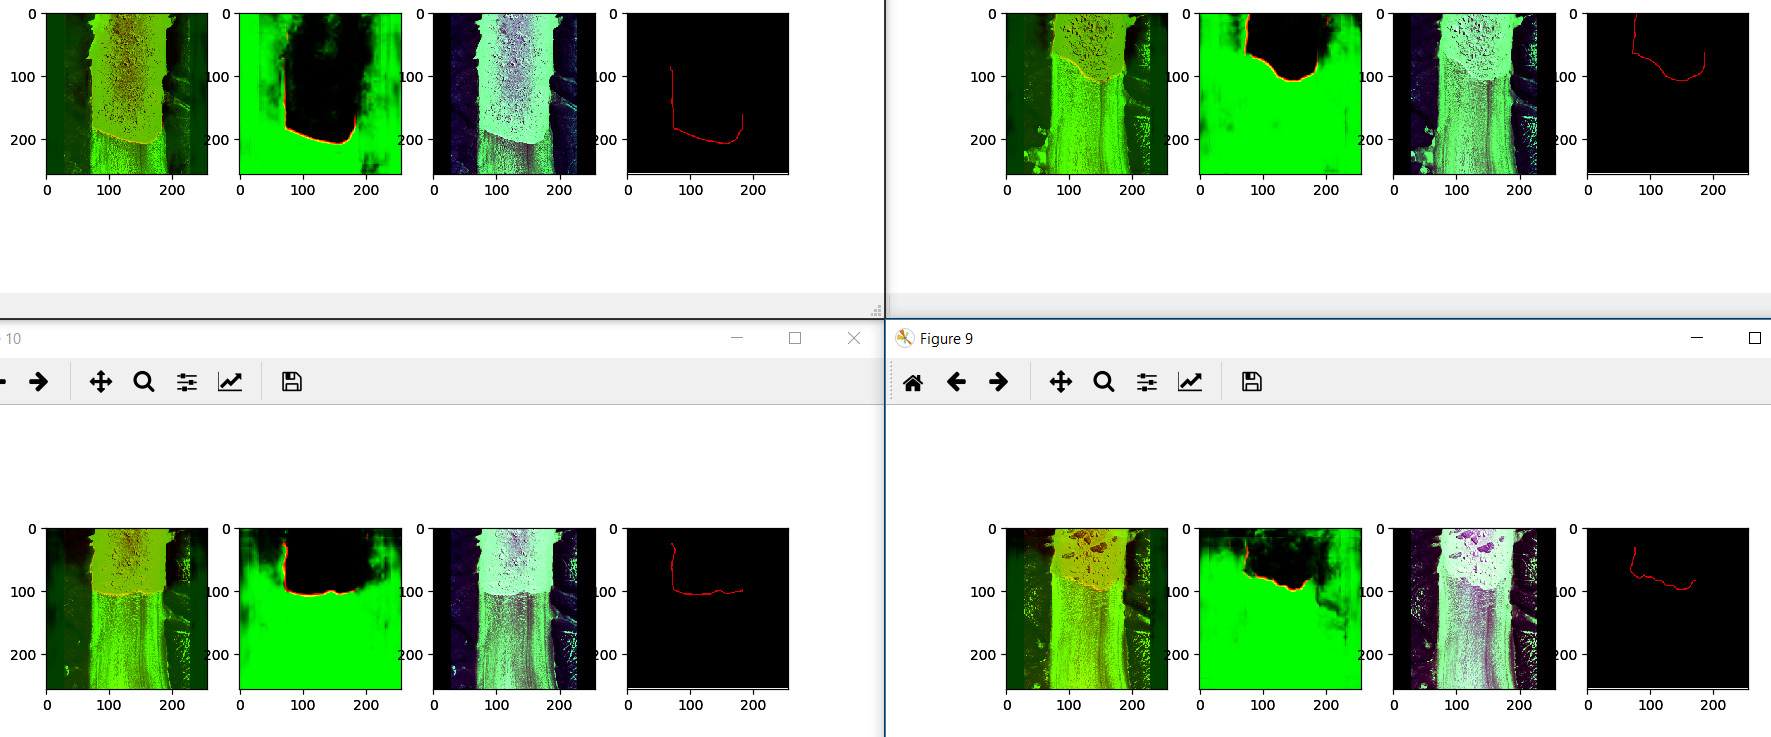
\includegraphics[width=18cm]{intercomp.png}
To be revised (add labels, compress, rescale). Left images are raw overlaid with prediction mask.
2nd images are predicted output from the network.
3rd images are the preprocessed raw images.
4th images are the isolated polylines.
\centering
\end{figure}
\begin{figure}[t]
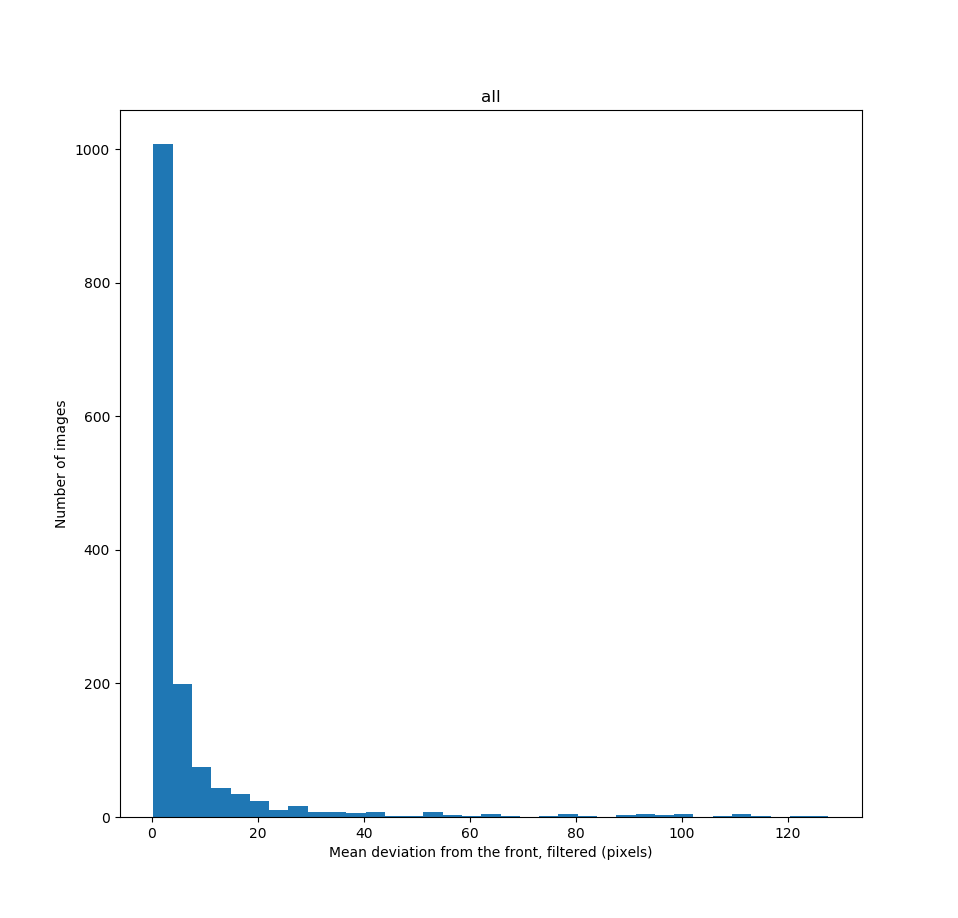
\includegraphics[width=18cm]{all_mean_deviation.png}
Mean deviation from the front, over all 192 validation images for 66 domains
\centering
\end{figure}
\begin{figure}[t]
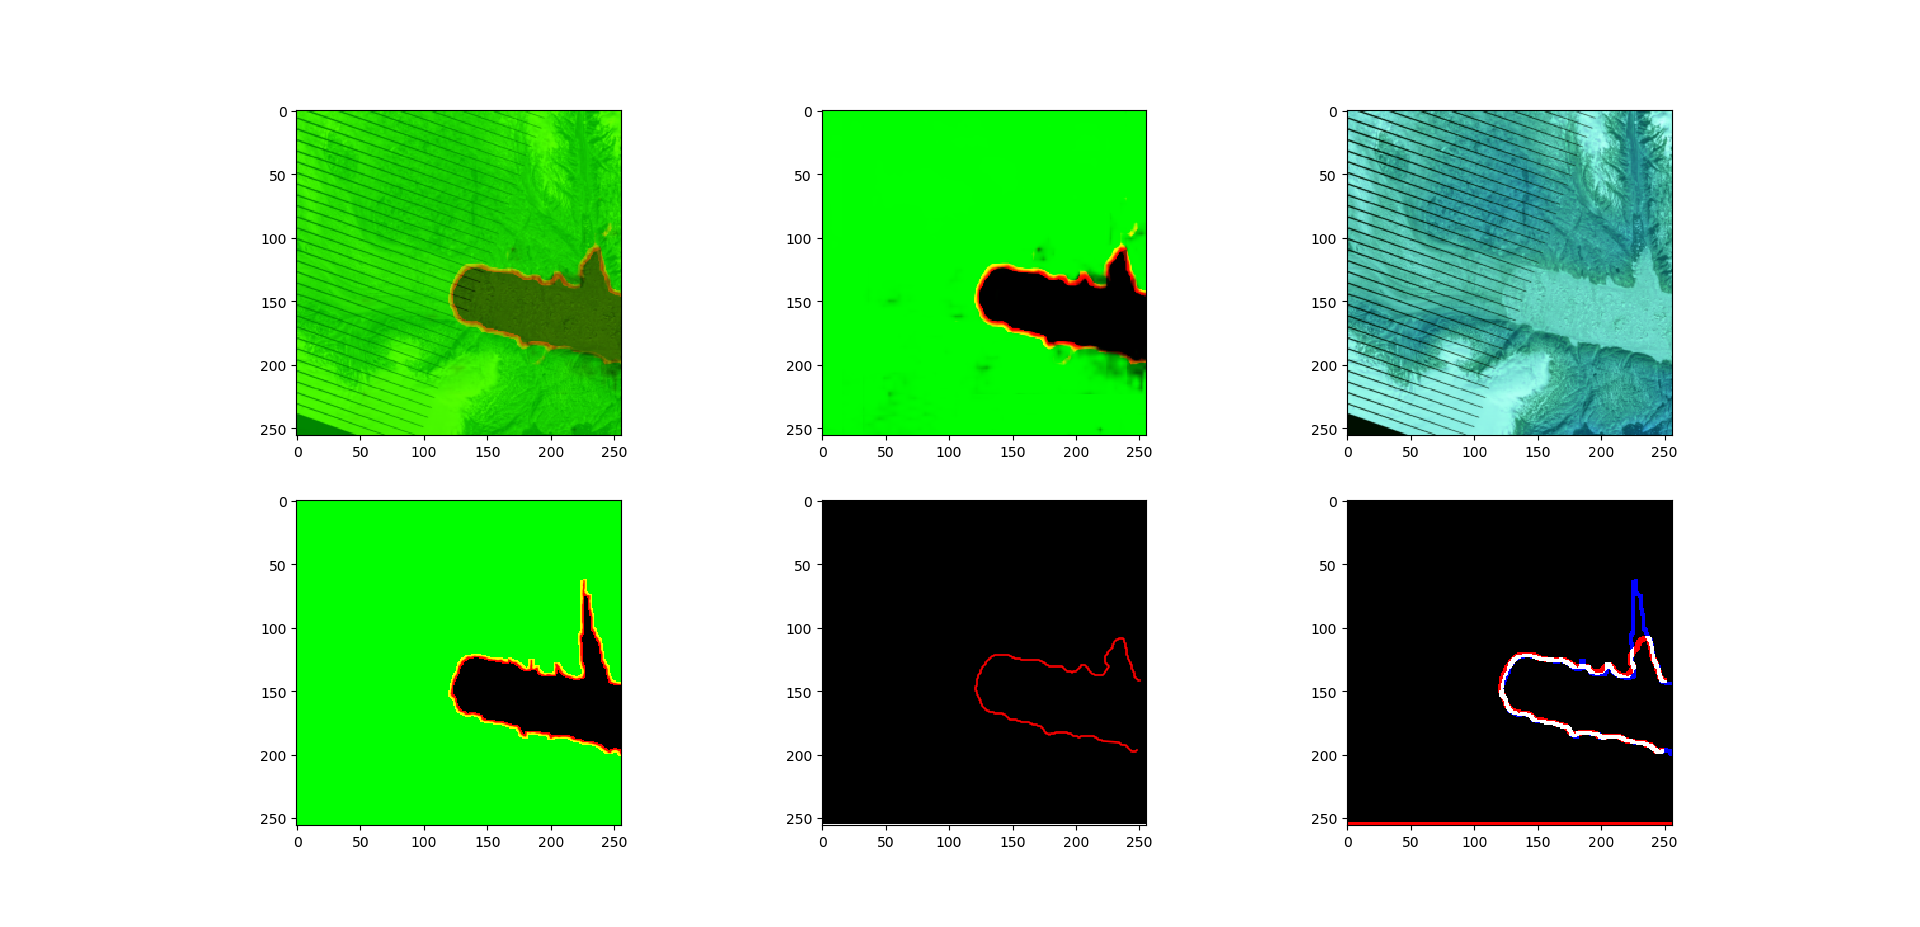
\includegraphics[width=18cm]{helheim_output.png}
To be revised (add labels, compress, rescale
\centering
\end{figure}
%Retrieve graphsfrom pyplot, showing mean deviation from front histograms
\subsection{Results - Data}
Approx 2k high res, hand-made/verified data (<30m accuracy from hand drawn line, but should be cross validated with other's data - see intercomparison section). Derived from training data. 66 domains, ~4-50 data points for each domain
Approx 20k unverified test data ~40-500 data points for each domain
Shapefile
\subsection{Results - Methodology}
We have two primary methods of evaluating the predicted output of any calving front against the ground truth labeling.
The first method is the standard Intersection over Union, or Jaccard score. This metric evaluates the degree of overlap between the predicted and ground truth pixel masks of the calving front. 

The second method is the domain specific Mean Deviation from the Front, which is conceptually similar to the technique utilized by Mohajerani et al.\cite{mohajerani-rs}. This metric evaluates the average distance from between closest points in the predicted and ground truth calving fronts. This metric is also evaluated in an alternative way. This method is to find the area of the intersection of the predicted and ground truth masks, and divide the length of the ground truth front.

51.36\% weighted IoU score (25/26 edge weight, 1/26 ice/ocean mask weight)
target: ~200m mean deviation from the front. min mean in Kangerlussuaq at ~1.5 pixels on validation set. What this network lacks in accuracy, it makes up for in generalizability - no other network has tested consistently on this number of domains.



\section{Discussion - Training the Neural Network}

Our work was performed alongside - and builds on - existing work done in the field.


\section{Discussion - Existing Work}
Our work was performed alongside - and builds on - existing work done in the field.

Mohajerani et. al.\cite{mohajerani-rs} provides a similar case study using the same type of deep neural network architecture to detect calving fronts. His study is performed on the Greenlandic glacial basins Jakobshavn, Helheim, Sverdrup, and Kangerlussuaq. Mohajerani's methodology displays promising steps towards generalizability and has been preeminent in the field.

Zhang, et. al.\cite{zhang-tc} performs an analysis similar to Mohajerani, albeit in a more specific case study using SAR data of Jakobshavn. The applicability of neural networks as a general methodology for calving front analysis is supported by its successful usage here. 

Baumhoer evaluates modified UNet architectures, as applied to SAR data of Antarctica. Her studies incorporate large spatial context in order to capture whole-coastline delineations. The prospect of larger networks on the order of 768x768 pixels offers the promise of higher resolution/accuracy outputs.

Our methodology shares the same basic approach with the above. We utilize an updated neural network architecture - DeeplabV3+ Xception - that improves upon the base UNet design. Furthermore, we use additional postprocessing steps to make the detection more accurate.

\section{Discussion - Inter-model Comparison}

We perform an inter-comparison between the performance of CALFIN with respect to the study conducted by Mohajerani et al. This ensures a robust and standardized way to compare disparate models and evaluation metrics.
To do this, we process the validation data used by each other's models, and compare the results.
%TODO
%have Yara/Mike insert results of preprocessed Helheim on Yara's network here?

%Will insert figure, similar graphs to Mohajerani et al. fig. 3
Across the all 10 test images in Mohajerani et al., we attain a 103.23 meter (2.11 pixel) mean deviation between the predicted and the ground truth fronts. We see that this approaches the level of accuracy achieved in the original study, which was 96.3 meters (1.97 pixels). While our method does not exceed this level of accuracy, it was still able to approach it with no further training done. We conjecture that the relatively higher resolution and the lack of wider context in the input image results in this performance gap.
To validate this conjecture, we reevaluate our Helheim validation images at higher resolution subsets, but with the added context of the nearby terrain and surroundings. %TODO

Overall, this inter-comparison supports our hypothesis that our methodology is generalizing well and is sufficiently accurate.

\section{Conclusion \& Future Work}
The calving front data products are being released on rolling basis at www.ics.uci.edu/~dlcheng. %datadryad or NSIDC?
The neural network model is being released on https://github.com/daniel-cheng/CALFIN.

Overall, we accomplished our goal of implementing a method for automatic delineation of calving front edges. Our method utilizes the cutting-edge in terms of deep learning architectures and techniques. We are able to achieve reasonable robustness to minor cloud cover, Landsat 7  scan line errors, illumination changes. We address issues with generalization through use of additional training data and an improved neural network architecture. We were competitive among existing work being done in this field.  

Our data augmentation, network architecture, and postprocessing methods all contribute to the success of our methodology. Ultimately, this work showcases the state-of-the-art in field of deep neural networks as applied to automated calving front detection, and provides a new database of calving fronts for the scientific community.


\subsection{Author contributions}
\subsection{Competing interests}
\subsection{Acknowledgments}

\bibliographystyle{unsrt} 
\bibliography{references}  %%% Use the external .bib file (using bibtex).

\end{document}





















%======================
%======================
% / __ \| |    |  __ \ 
%| |  | | |    | |  | |
%| |  | | |    | |  | |
%| |__| | |____| |__| |
% \____/|______|_____/ 
%======================
%======================
%\section{Methodology - Evaluation}
%Skip to Implementation - may eliminate evaluation/"story" of evaluation
%\subsection{Methodology - Evaluation}
%We evaluated a variety of processing methods, ranging from: naive edge detection; %to texture filter analysis; and ultimately, convolutional neural networks (CNNs). %Our study reveals a natural progression of how each method builds upon the previous %ones, and sheds light on how CNNs naturally incorporates the previous methods to %achieve better performance.
%
%\subsubsection{Edge Detection}
%Our initial efforts led us to begin testing basic edge detection on Landsat imagery %in order to automatically detect calving fronts. We used Canny-edge filtering [1] %to generate a list of edges, and  and additional processing algorithms to prune %small/erroneous edges from the filtered image.
%\textbf{Pros}
%This method is straightforward to understand, easy to implement, and fast to %evaluate.
%\textbf{Cons}
%However, this method suffers from inadequacies. It is not robust with respect to %ice mélange, illumination changes, clouds, and Landsat 7 scan-line errors. %Additionally, the necessity of removing small/erroneous edges introduces error due %to the inability of line processing algorithms' ability to discern "correct" edges.
%
%In the end, we were only able to achieve low accuracy classifications of the edge. %Edge detection alone is insufficient for this task, It does not utilize the full %breadth of information available needed, and more robust methods are required.
%
%
%\subsubsection{Texture Analysis}
%A new filtering method was needed, and texture analysis suited the requirements. At %its core, this method utilizes a set of convolutional image kernels, or filters. %These filters are applied to the input to create a feature map. Each pixel will %thus have an associated feature vector, with values associated with the activation %for each unique filter in the set. Note that these filters may detect features such %as edges, and this method is thus an extension of the previous one.
%
%Subsequently, a family of machine learning techniques - unsupervised learning - may %be applied to these feature maps. This allows for the classification of closely %grouped feature vectors, which correspond to semantically similar textures.
%
%\textbf{Pros}
%In our implementation, we perform feature vector generation via Gabor + Gaussian %filters. We perform pixel-level classification via K-means clustering and Support %Vector Machines/Error Correcting Output Code models. We found k-means to be less %performant with respect to SVM/ECOC modeling. Note that training the SVM/ECOC %models requires ground truth, which we generated ourselves.
%
%\textbf{Cons}
%Unfortunately, this method is still inadequate, and while more robust to %illumination changes, it was still unable to account for scan-line errors, ice %mélange, and clouds. 
%
%To surpass these limits, another processing paradigm needed to be found.
%
%
%%Rewrite this section
%\subsubsection{Neural Networks}
%Thus we arrive at the state-of-the-art in machine learning classification: neural %networks. We utilize the convolutional neural networks (CNNs), which are image %oriented NNs that are efficient to evaluate and train. CNNs build upon - and are %the logical progression of - texture filtering. To achieve even better accuracy and %robustness, CNNs automatically learn the best image filters to use, and are able to %utilize higher order filters to extract high-level, abstract features that %approximate human visual processes.
%
%\textbf{Pros}
%The CNNs we utilize have good generalization and discrimination capabilities. They %are able to "look past" Landsat 7 scanline errors, light cloud cover, and %illumination changes. They are able to capture fine detail such as ice tongues and %ice melange. Furthermore, it is robust with respect to different %resolutions/scales. Moreover, it can handle noise/errors in the data, such as the %forms found in Landsat 2 imagery. 
%%Include examples here?
%We are also able to perform additional preprocessing - data augmentation - on the %inputs. This allows us to ensure minor perturbations to the input still result in %the same output. This prevents the over-fitting or memorization of the training %set, and ensures the network generalizes to other glacial domains.
%
%\textbf{Cons}
%Neural networks are computational expensive and time consuming to train. They may %be seen as "black boxes" as well due to their obfuscated inner models - it is not %apparent what the NN is "seeing" without extraneous effort. Additionally, neural %networks require large amounts of ground-truth/training data. Due to the specific %requirements of accuracy and input format, we were not able to use publicly %available data from ESA-CCI, or other individual sources of calving front %locations. %(i.e., from Sophie Gallagher, James Lea, Stephen Baxter).
%Therefore, it was required to manually delineate our own training data. This was a %time consuming, if not accurate method of assimilating the required data.
%.
%.
%.
%
%\pagebreak

%\subsection{Analysis}
%
%
%\begin{table}[ht!]
%\centering
%\caption{Architecture Evaluation}
%\label{tab:table-arch-eval}
%\begin{tabular}{ll}
%Architecture               & Best IoU \\
%UNet 256 32-4-2            & 0.3802   \\
%Deeplabv3+ MobileNetV2 224 & 0.6956   \\
%Deeplabv3+ MobileNetV2 256 & 0.6026   \\
%Deeplabv3+ Xception 224    & 0.8794   \\
%Deeplabv3+ Xception 256    & 0.8986   \\
%Deeplabv3+ Xception 384    & 0.8257   \\
%Deeplabv3+ Xception 512    & 0.6956  
%\end{tabular}
%\end{table}
%
%\subsubsection{Model }
%\subsubsection{UNet 256 32-4-2 }
%We began our evaluation with a classic UNet architecture \cite{unet}. We %chose an input size of 256 by 256 pixels. This size was chosen to %encompass a small majority of available glacial basin domains within a %single image. We chose the number of first-layer feature maps to be 32, a %depth of 4 layers, and a feature multiplier of 2 per layer. 
%
%While this architecture proved to be a good start, it did not have the %capacity to robustly classify glacial calving fronts. It suffered %primarily from an inability to robustly discriminate against ice melange, %which greatly impacted its performance. Additionally, modification of the %hyper-parameters (input size, feature map number, depth, feature %multiplier)
%
%Validation best IoU: 0.3802
%Test best IoU:
%
%\subsubsection{Deeplabv3+ MobileNetV2 224}
%This capacity limited
%Validation best IoU: 0.6956
%Test best IoU:
%
%
%\subsubsection{Deeplabv3+ MobileNetV2 256}
%worse performance, but still capacity limited, and could be trained %further, but not promising
%Validation best IoU: 0.6026
%Test best IoU:
%
%\subsubsection{Deeplabv3+ Xception 224}
%very good, better than both MobileNetV2 backbones, and best so far.
%However, low spatial resolution.
%Validation best IoU: 0.8776 ( verify 0.9695)
%Test best IoU:
%
%\subsubsection{Deeplabv3+ Xception 256}
%worse performance, better spatial resolution. Seems to be capacity or %data limited.
%Validation best IoU: 0.8986
%Test best IoU:
%
%\subsubsection{Deeplabv3+ Xception 384}
%worse performance, better spatial resolution. I believe the field of view %is now too large.
%Validation best IoU: 0.8257
%Test best IoU:
%
%\subsubsection{Deeplabv3+ Xception 512}
%worse performance, better spatial resolution. Field fo view is too large. %Need to capture finer detail. Perhaps can use conv layers to resize.
%Validation best IoU: 0.5723
%Test best IoU:
%
%Training regimen:
%~5075 seconds per epoch
%4000 iterations per epoch
%500 batches per epoch
%2 images per iteration
%8 iterations per batch
%16 image batch size
%
%\section{Postprocessing}
%\subsection{Incorporating Time Series Information}
%The output of the neural network is improved over naive approaches, but %it still lacks information from adjacent time series imagery. Since this %application demands accuracy, we study different methods of incorporating %temporal information into the output.
%\subsubsection{Raster Mask to Vector Line Representation}
%The first step we take is to utilize OpenCV, a library of computer vision %methods. We use OpenCV to transform binary mask images into vectorized %poly-line segments. At this stage, deficiencies in the mask may result in %multiple separated line segments. 
%
%\subsubsection{Wiggle-line algorithm - Simplified Simulation of Calving %Front Evolution}
%The next step we take is a unique strategy, in which we perform a naive %simulation of the evolution of the front. In order to do this, we process %each domain from the first available time step to the last, in order. %\textbf{We manually delineate the first time step} in each domain to %ensure our initial value is as accurate as possible. Subsequently, we %re-process the next mask in the time series using the distance transform. %This produces a gradient map, where each pixel contains the direction %towards the closest point in the estimated calving front mask, and a %magnitude corresponding to the distance from said point. We then treat %this problem as an optimization problem, wherein each point in the %calving front in the first time step can minimize its energy in the %subsequent time step's gradient map. This method allows for robustness to %deficiencies in the binary mask - i.e., holes in the detected front will %be effectively "skipped" during this optimization step, as the points %around this hole will still be connected given correct initialization. %Subsequently, the polyline is re-sampled to redistribute the points %evenly along the line to avoid degeneracies.
%
%The above steps can be then repeated for each following time step, until %all time steps for the single glacial basin are processed.
%
%\subsubsection{Shapefile Generation}
%Once all the masks have been processed into polylines, they can be %transformed into Shapefiles. To do this, we reference the original %GeoTIFF image subset generated during preprocessing. From here, a simple %coordinate transformation and reprojection allows us to write the %associated Shapefile materials. We provide the calving front in both %polygon and line formats. Additional processing can be done to eliminate %the static coastline from the provided fronts.
%
%\subsubsection{Regarding the potential usage of Recurrent Neural %Networks}
%Given the temporal nature of this data, it is natural to assume use of %Recurrent Neural Networks for the primary prediction step. However, this %approach raises several concerns.
%1. The dataset is temporally irregular. Unlike current video-based %analysis networks, inter-frame gaps for satellite imagery are %unpredictable, and can vary due to satellite availability, seasonal %illumination restrictions, and cloud cover. These gaps can range among %almost 2 orders of a magnitude, from 10 days to several months and even %several years among earlier datasets.
%2. The benefit is not perceived to be beneficial to a degree that it is %worth pursuing over other more efficient, and more sustainable methods.
%3. Lack of available training data. While it data augmentation in the %spatial domain is heavily used, data augmentation in the temporal domain %does not present a clear approach, and would instead rely on 
%4. The learned representation is hard. A human would find it hard to more %accurately predict the output given 3 temporally similar images over 1. %This is given the unpredictable nature of events such as calving.
%5. Such a network would not be readily generalizeable. Since network %would be learning basin-specific front movement, it would not be very %applicable to new glacial basins.
%
%At this point, while it is possible for the network to learn %annual/decadal trends, it is uncertain whether or not it can make use of %this information in a meaningful way such that accuracy is improved. Thus %we do not pursue the usage of RNNs in our current iteration of CALFIN.
%
%
%\section{Results \&  Error Analysis}
%\subsection{Upernavik}
%Able to capture glacial tongues
%Uses texture gradient to detect ice mélange boundary
%
%\subsection{Jakobshavn}
%Ice mélange causes uncertainty
%Manageable with postprocessing
%Compression/scaling may decrease accuracy
%
%\subsection{Hayes}
%Extra training allows ice mélange to be more clearly separated
%Not as consistent due to complexity of fronts
%
%\subsection{Kong-Oscar}
%Worst accuracy all around
%Requires additional training
%
%\subsection{Kangiata-Nunata}
%Handles light cloud cover/Landsat 7 scanline errors
%Shows signs of overfitting/memory effects
%
%\subsection{Rink Isbrae}
%Some images need to be manually labeled and retrained on
%
%\subsection{Docker-Smith North}
%Sparsely trained
%Calving events handled well
%Higher texture contrast, higher confidence
%Key goal: generalization
